%\subsection{System Demo}
%The architecture of our system is similar to that of OSM itself. 
%Our map data is stored on PostgreSQL, which provides strong support for
%geospatial data in an extension called PostGIS. 
%%The reason for selecting this database software for all of our crucial map data is because it is really one of the fastest and most state-of-art database, most importantly with strong support of geospatial database extension, PostGIS. Such extension comes extremely handy with some functions in SQL to help ease the pain of querying spatial data as well as spatial index for speedups. 
%The backend for providing map editing (with fronted application in JavaScript 
%called iD), showing slippy maps~\footnote{Slippy map is an OSM term that refers
%to maps that can be dragged around and zoomed in and out.}, 
%and the map API are from the OpenStreetMap's 
%Rails Port project (see \url{http://github.com/openstreetmap/openstreetmap-website}). 
%We simply run an instance of this backend at our own server, 
%and it uses our own database for data source. The OSM API is a REST web service 
%interface for reading and writing to the database i.e. XML over HTTP.
%%with use of simple URLs for object access, and standard HTTP response codes. Other OSM components access the database via this interface. It is also available to the outside internet. The API logic is all part of the same Ruby on Rails application which powers the OSM front end website.
%Another part of our system are the map rendering engine that serves 
%the latest map in form of tile images (similar to Baidu map). 
%%so that the frontend could have beautiful cartography. 
%The main backend for the rendering the maps is Mapnik 
%(see \url{http://mapnik.org/}).
%%There are several great open source utilities provided by OpenStreetMap that is really useful for converting and processing the downloaded data from data dump sites and used in scheduled jobs to exporting and importing updated data from API database to the PostGIS database used by Mapnik for tile rendering, which include Osmosis, an OSM data processing Swiss army knife, and OSM data importer for rendering or geo-coding, osm2pgsql, a powertool for importing OSM XML files into PostGIS databases.
%Finally, the prediction engine is a servlet application running on
%Tomcat. The demo web frontend uses the Leaflet.js library 
%(\url{http://leafletjs.com/}). \figref{fig:demoresult}
%show the web demo interface and a prediction of a small area in Shanghai.
%
%%\begin{figure}[th]
%%\centering
%%\resizebox{\columnwidth}{!}{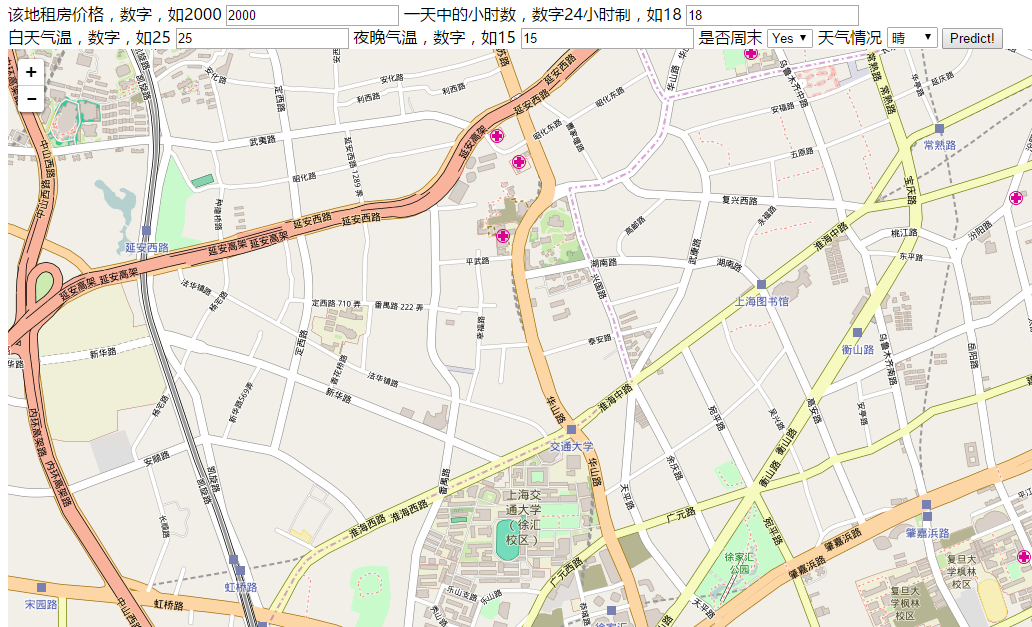
\includegraphics{figures/implementation/frontend.PNG}}
%%\caption{Frontend demo page}
%%\label{fig:demo}
%%\end{figure}
%
%\begin{figure}[th]
%	\centering
%	\resizebox{\columnwidth}{!}{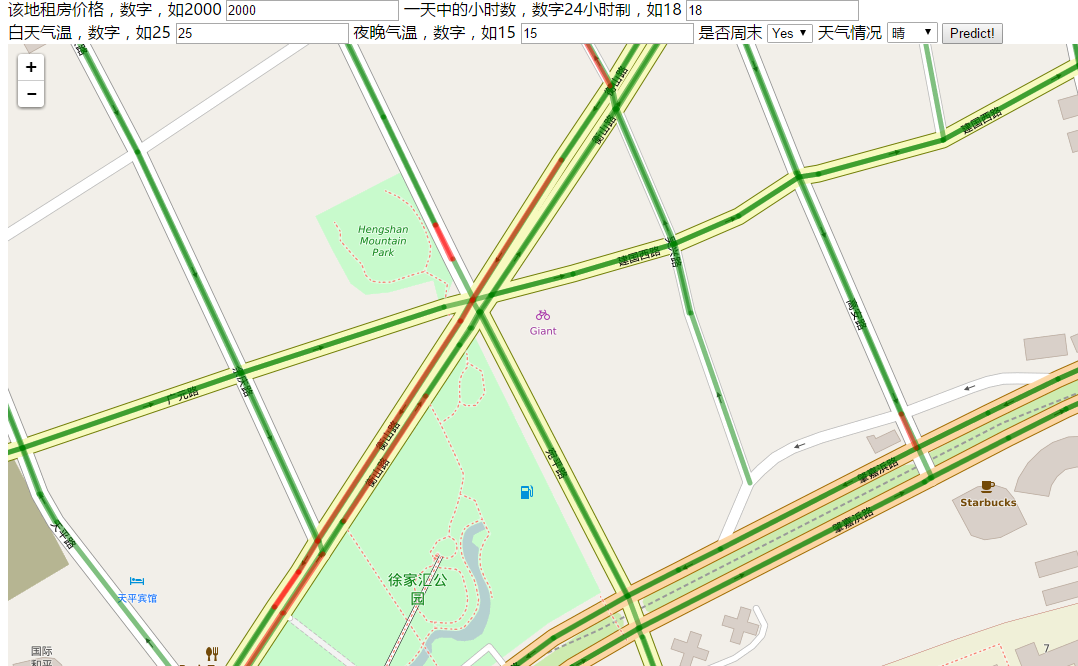
\includegraphics{figures/implementation/demo_predict.PNG}}
%	\caption{Frontend demo prediction result page}
%	\label{fig:demoresult}
%\end{figure}
%
%
%%The server where we are running all these system components is powered by 
%%Ubuntu 12.04.5 LTS, with Intel Xeon(R) CPU E5504 CPU and 48 GB of memory.
%%\begin{figure}
%%	\centering
%%	\resizebox{\columnwidth}{!}{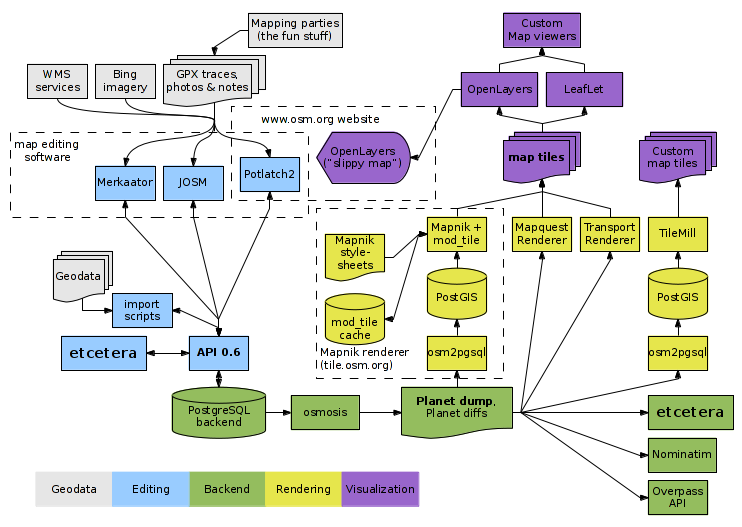
\includegraphics{figures/implementation/OSM_Components.png}}
%%	\caption{OpenStreetMaps software stack and components}
%%	\label{fig:osmcomponet}
%%\end{figure}
%	
%%\subsection{Map Database}
%%The map database is one of the most important part in our system because it stores all the information we previously obtained. The map database is also called the main database since obviously it is where we keep all our data. The main database is accessed for editing via the API, so the editing is also made in this database. The database contains tables for each element type (nodes, ways, relations). In fact, for each of these there are several database tables: current, history, current\_tags, history\_tags. In addition, there are database tables for storing changeset, gpx\_files, users, diary entries, sessions, oauth etc. The database contains several tables and relations that is shown it the figure. The database we used is PostgreSQL, with strong geospatial capabilities. PostgreSQL has geometry types. For our core OSM database we do not use these. We have own representation of OpenStreetMap data primitives. The PostGIS extension for PostgreSQL is often used for geographic data. PostGIS adds geospatial functions and two metadata tables. Again we do not use this for our core database, however we do use all of these things on the tile server database as required by the Mapnik rendering engine. Osmosis can be used to populate a more general PostgreSQL/PostGIS database from a OSM data dump file, where we initially populated and loaded the Baidu POIs. We also added some other geographic related functions and data types to our instance of database, such as proximity querying, etc. A changeset, as you can see in both database schemas and OSM XML files, consists of a group of changes made by a single user over a short period of time, for example someone edited the map in a session of urban planning process. One changeset may for example include the additions of new elements to OSM, the addition of new tags to existing elements, changes to tag values of elements, deletion of tags and also deletion of elements. The ER-diagram is shown in Figure~\ref{fig:erdiagram1},~\ref{fig:erdiagram2} and~\ref{fig:erdiagram3}, the most important tables are \textit{current\_nodes/nodes, current\_ways/ways, current\_node\_tags/node\_tags} as well as \textit{current\_way\_nodes/way\_nodes}. Those are the table we used most frequently because they hold our map data primarily. Those columns named k and v are just representing the tags in the form of key-value pairs. Several of indexes and foreign key on columns on tables exist, refer to the DDL statement for more details.
%%\begin{figure}
%%\centering
%%\resizebox{\columnwidth}{!}{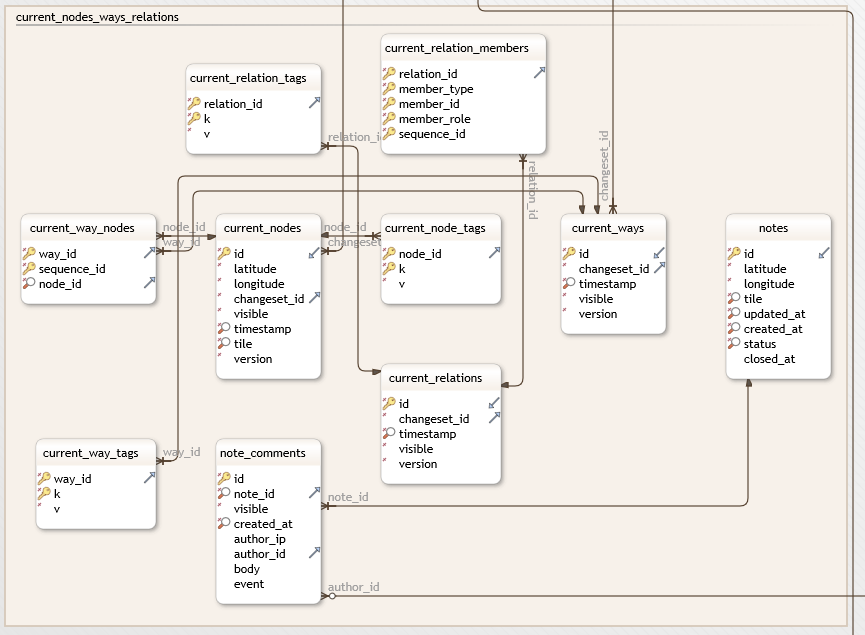
\includegraphics{figures/implementation/current_nodes_ways_relations.PNG}}
%%\caption{Main database ER-diagram part 1}
%%\label{fig:erdiagram1}
%%\end{figure}
%%\begin{figure}
%%\centering
%%\resizebox{\columnwidth}{!}{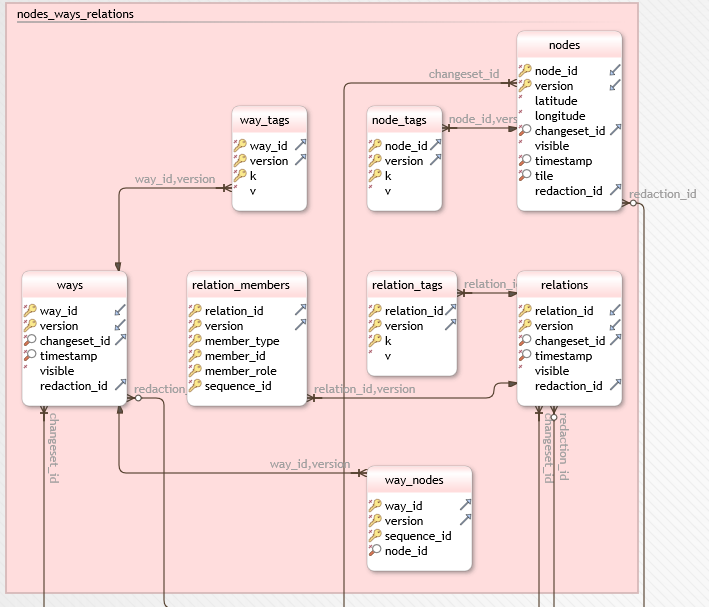
\includegraphics{figures/implementation/nodes_ways_relations.png}}
%%\caption{Main database ER-diagram part 2}
%%\label{fig:erdiagram2}
%%\end{figure}
%%\begin{figure}
%%\centering
%%\resizebox{\columnwidth}{!}{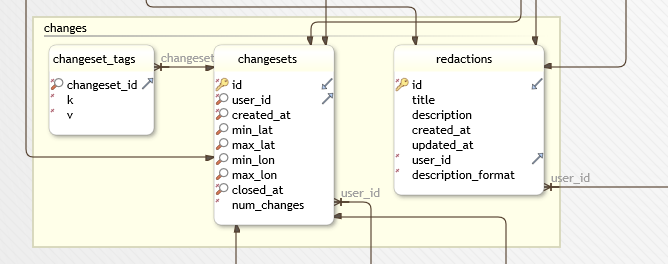
\includegraphics{figures/implementation/changes.PNG}}
%%\caption{Main database ER-diagram part 3}
%%\label{fig:erdiagram3}
%%\end{figure}
%%				
%%\subsection{Tile Rendering}
%%The process of rendering a map generally means taking raw geospatial data and making a visual map from it. Often the word applies more specifically to the production of a raster image, or a set of raster tiles, but it can refer to the production of map outputs in vector-based formats. ``3D rendering" is also possible taking map data as an input. The ability to render maps in new and interesting styles, or highlighting features of special interest, is one of the most exciting aspects having open access to geo-data. Developers in and around the OpenStreetMap community have created a wide variety of software for rendering OpenStreetMap data. The data can also be converted to other data formats for use with existing rendering software. The rendering engine we used to provide those beautiful tile maps is called Mapnik. Mapnik is an open source toolkit for rendering maps. Among other things, it is used to render the five main Slippy Map layers on the OpenStreetMap website. It supports a variety of geospatial data formats and provides flexible styling options for designing many different kinds of maps. Mapnik is written in C++ and can be scripted using binding languages such as JavaScript (Node.js), Python, Ruby, and Java. It uses the AGG rendering library and offers anti-aliasing rendering with subpixel accuracy. Mapnik can use data from different sources: it can directly process OSM data, PostGIS databases, shapefiles and more. In our system design, PostGIS database is used, with data updated from the main database we introduced earlier. PostGIS is the most common approach for rendering OSM data with Mapnik. OSM can be loaded by a tool such as osm2pgsql or Imposm and accessed via SQL queries and GIS functions defined in a Mapnik style. This approach can be used for more advanced renderings, and is the main datasource used by the Standard OpenStreetMap layer. Mapnik allows for customization of all the cartographic aspect of a map - data features, icons, fonts, colors, patterns, and even certain effects such as pseudo-3d buildings and drop shadows. This is all controlled by defining datasources and style rules, most commonly in an XML language specific to Mapnik. The style we used is the same as the OpenStreetMap standard one, which is open source and beautiful (written in CartoCSS supported by Mapnik, \url{https://github.com/gravitystorm/openstreetmap-carto}). The Figure~\ref{fig:mapnikexample} shows the style used.
%%\begin{figure}
%%\centering
%%\resizebox{\columnwidth}{!}{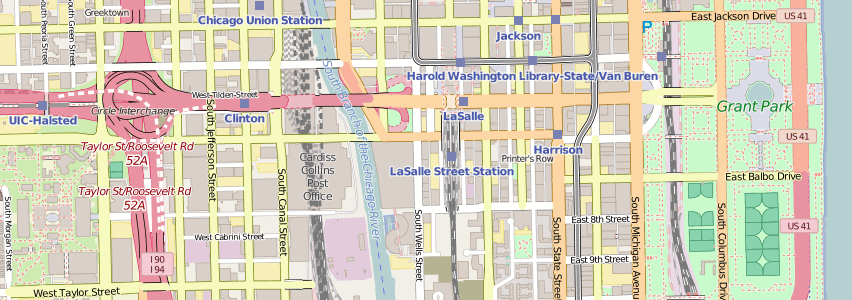
\includegraphics{figures/implementation/mapnik_example.png}}
%%\caption{An example rendering using Mapnik with OpenStreetMap carto style}
%%\label{fig:mapnikexample}
%%\end{figure}
%%
%%\subsection{Prediction Engine}
%%This is the most important part in the whole project and is very crucial and special. It is a servlet program written in Java, as a Servlet and running in the very popular Tomcat Servlet container. The prediction engine listens at a HTTP port and accept requests with given parameter. It is running with URL pattern /prediction and with query parameters x1, x2, y1, y2 representing the bounding box longitude and latitude of the prediction area, as well as the hour representing the hour of the day ranging from 0 to 24, and price representing the average house rental price of the requested area, along with day\_temp and night\_temp, representing the temperature of day and night. After some calculations and processing, the prediction engine responds with a large JSON format data, containing list of 5-tuples, each with the form of (starting coordinates, ending coordinates, predicted traffic situation). Every two consecutive nodes in one way will form such a tuple representing a road segment, the smallest unit of prediction. In cases of one-way road, only one tuple exists for one such segment, and in cases of two-way road, two tuples exist for one such segment, with starting coordinates and ending coordinates exchanged, and with new predicted traffic situation.
%%
%%During this process, the program mainly does a few things in steps to be clear. Firstly, the Servlet program called prediction.java receive the request and parse the parameter described above, getting the bounding box and some other designated parameters for prediction. Then the program access the main map database introduced above, querying the \textit{current\_nodes, current\_ways} and \textit{current\_way\_nodes} table with the condition that only nodes and ways within the bounding box get selected. After successfully getting the query result, the map data is stored in an object with all the connections and relations as Map data structure in Java. A method named organizeWays is called to organize queried ways and nodes into the right sequence and become connected. Then begins the data preprocessing to achieve the input data in required format for LIBSVM. First generate the crossings of the roads and calculate all the features related to crossings by the class named genCross and calCross. We calculate the crossings several blocks ahead and behind, following the same rule that was used in previous training and testing experiments, storing data in feature result list. After that, the program begins to search and count the number of points of interests of all types predefined and derived from Baidu types. As stated in data collection chapter, all the POIs have been imported into the main database’s \textit{current\_nodes/nodes} table with specific tag poitype=*, so with the help of the strong and robust spatial functionality that PostgreSQL database provides, we can use SQL queries to easily search all the points within a given radius of the given coordinates. It is achieved by Cube and EarthDistance, and these 2 extensions provide easy to use and very fast methods to accomplish some more minor geo related activities. Before doing anything, we prepared the database with two lines of SQL to create such extensions:
%%\begin{lstlisting}[language=SQL, caption=Create required extension in PostgreSQL]
%%CREATE EXTENSION cube;
%%CREATE EXTENSION earthdistance;
%%\end{lstlisting}
%%Query and get a set of all POI types that exist in our database:
%%\begin{lstlisting}[language=SQL, caption=Query all POI types]
%%SELECT * FROM current_node_tags WHERE current_node_tags.k='poitype';
%%\end{lstlisting}
%%
%%And then, at the beginning of each request, we create a temporary table called poi\_nodes out of only POI nodes that have necessary tags inside, so that the search later would be in a much smaller range of data.
%%
%%\begin{lstlisting}[language=SQL, caption=Create temporary table poi\_nodes]
%%CREATE TEMPORARY TABLE poi_nodes ON COMMIT PRESERVE ROWS AS SELECT * FROM current_nodes WHERE current_nodes.id IN (SELECT current_node_tags.node_id FROM current_node_tags;
%%\end{lstlisting}
%%
%%And we created a spatial index using GiST on latitudes and longitudes of each node for it on the fly. GiST stands for Generalized Search Tree. It is a balanced, tree-structured access method, that acts as a base template in which to implement arbitrary indexing schemes. B-trees, R-trees and many other indexing schemes can be implemented in GiST. The advantage of GiST is that it allows the development of custom data types with the appropriate access methods, by an expert in the domain of the data type, rather than a database expert. So we can be sure that what we are querying is all about longitude and latitude. Though making this index in context of the whole Shanghai area would take more than one or two seconds, it is worth the trade off because after my experiment, with index each radius search query would take nearly 2 seconds to complete the sequential search and heavy calculating each row. After the indexing, each query takes about 20ms to complete, which is a great improvement. Note that the longitude and latitude in the database are being multiplied by 1e7 as an integer, so here we shall divide it back to normal double.
%%
%%\begin{lstlisting}[language=SQL, caption=Create index on table poi\_nodes]
%%CREATE INDEX on poi_nodes USING gist(ll_to_earth(poi_nodes.latitude * 1.0 / 1e7, poi_nodes.longitude * 1.0 / 1e7));
%%\end{lstlisting}
%%
%%Then comes the interesting part. Because we have a lot of nodes from all ways in the area, the search is quite extensive. Each node that belongs to a way has a feature with the counting of how many points of interest of given type are there in vicinity of the node, and add those numbers to the feature list of every node. This is where the previously created extension comes useful. The two of the many functions we use here is calculating the distance between coordinates and finding records in a radius. To calculate the distance between 2 coordinates we use \textit{earthdistance(lltoearth(\$latlngcube), lltoearth(\$latlng\_cube))}. This function allows us to pass 2 sets of coordinates and it will return a numerical value representing meters. Another great function provided by these extensions is \textit{earth\_box(ll\_to\_earth(\$lat, \$lng), \$radius\_in\_metres)}. This function allows us to perform a simple compare to find all records in a certain radius. This is done by the function by returning the great circle distance between the points. The following is the actual query that run for each node and each type to be counted. The searching radius is 200 meters in our case.
%%
%%\begin{lstlisting}[language=SQL, caption=Query the POIs in range]
%%SELECT * FROM poi_nodes WHERE earth_box(ll_to_earth(lat, lon), radius) @> ll_to_earth(poi_nodes.latitude * 1.0 / 1e7, poi_nodes.longitude * 1.0 / 1e7);
%%\end{lstlisting}
%%
%%After iterating through all the nodes to query the points of interest around each given node. We managed to get those POI related features calculated and stored in format for later use.
%%
%%The next step in the whole prediction process is to prepare those calculated and queried features into prediction test data in order. It iterates through all the ways that previously visited in order, and look up relevant nodes within each way, extracting all the related items and features. For the first iteration process, it deals with the forward direction and in the second it deals with the backward direction. During the process, each feature line is written into a text file in the original order preserved so that later on the prediction process could output readable results. It is basically a file with many lines as the whole test data set, each line contains node ID and all the features used. Here is the end of the feature extraction process.
%%
%%When the next step of the real prediction starts, firstly the data set scale procedure provided from the LIBSVM library is invoked, with the same scaling parameters as the ones used in the training data set and model so that the consistency of data normalization could be achieved. After scaling all the testing data’s feature value right, the predict program from the open source LIBLINEAR is called for high speed prediction of the test data with given SVM model file. It takes the normalized data input for best result and the output is redirected to a text file. This process is actually relatively fast due to the high performance. It cost less time than the most time consuming data processing and feature extraction steps.
%%
%%As for the last step of returning and responding the predicted traffic situation of all roads back to the client, the prediction Servlet needs to read the test result and read the result in the same order as before when it is written. Because of this, it is trivial to save those predicted results along with the nodes' information and the consecutive nodes’ segments for later drawing in the frontend. Now we simply attach the starting coordinates and the ending coordinates together with the predicted traffic on this segment, and the one-way and two-way situations are treated separately. The case of the two-way roads actually becomes really tricky because we need the frontend to draw distinguishable lines of possibly different color (the traffic situation on each direction of the roads may vary largely due to many issues). The lines could not just have their starting coordinate and ending coordinate exchanged, because that would result in an exactly overlapped two lines in the same place with different color, causing the user not being able to distinguish. To solve this, we have to make a little bit of the offset to the second instance of the road segment representing the opposite direction. That is, when coming across the backward direction, we calculate the starting and ending coordinates using the linear parallel offset formula as we consider the longitude/latitude coordinates is equivalent to Descartes Coordinates in such a small area on earth. We neglected the fact that the earth’s surface is a sphere. By offsetting 1 to 2 meters distance to the original segment vector, the result is already distinguishable between two directions.
%%
%%However, regardless of those variants, the final result is a JSON file containing a list object containing a list of all the 5-tuples to be drawn. The response is then sent back the requesting client for later process. This is all the process that our prediction engine would do, it is still quite slow when adding all this together and one of our future work is to improve the response time.
%%					
%
%%Each application needs a good and useful interface to function properly. In our frontend page, it is made up of only one HTML file, along with several open source JavaScript libraries. The appearance is not fancy nor extensive for users, but it shows some of our system’s most import usage, which is predicting under the condition of current data and time and weather. The editing interface has a separate page and link, currently not customized and we simply use the iD online OSM map editor provided by OpenStreetMap and included in the Rails Port project which we have been running on our own server and introduced earlier. The demo page of the prediction we wrote is based on a very popular open source online mapping library called Leaflet.js (\url{http://leafletjs.com/}) which could be able to handle our own customized tile server and draw the prediction results in each color as polylines on the tile map layer. Leaflet is the leading open-source JavaScript library for mobile-friendly interactive maps. Weighing just about 33 KB of JS, it has all the mapping features most developers ever need. Leaflet is designed with simplicity, performance and usability in mind. It works efficiently across all major desktop and mobile platforms, can be extended with lots of plugins, has a beautiful, easy to use and well-documented API and a simple, readable source code that is a joy to contribute to, and that is why we choose to use it because it is really strong and small in size. On the page there are several input boxes and dropdown selections that allows the user to input the scalar parameters that needs to be provided by the user. Below the input form is where the Leaflet library comes into use. There is a slippy map interface that allows the user to freely zoom in and zoom out as well as pan around to browse the map. The tile image layer is defined while creating the class with our own Mapnik rendering server. After the user put the desired area into the screen size, he or she would click on the predict button with all the parameter input. The frontend code would retrieve the longitude and latitude of the bounding box that the map currently shows, checking the zoom to see if it is too big an area that would cause potential crash. Then, along with all the input data after checking validity, all those parameters are retrieved from the frontend page and the page would send a AJAX HTTP request to the prediction engine’s listening URL. This will initiate a prediction process and while waiting for response, the frontend web page shows up a notification popup modal indicating that it is currently running. After the data is received and all the road segments, three new multi-polyline layers are initialized and pushed all lines with different prediction results represented in different colors defined earlier into the layer’s lists respectively. The lines contained the longitude and latitude starting and end point data, inserted into the layer with the right color by switching on the predicted result. Then the layers loaded with data are attached to the map object, so that the result could be shown on the web page in correct colors. A quick note is that all the traffic prediction results is drawn on the client side in browser by JavaScript. It turns vector data format into the images, so the performance requirement is actually quite heavy, so limiting the rendering area is necessary. This explains the whole process that the frontend does, basically only calling the backend prediction engine to get the test result and draw the result on top of the map by using the Leaflet.js library’s tile layers and vector layers’ functionality. See Figure~\ref{fig:frontenddemopage} for user interface and Figure~\ref{fig:frontenddemoresultpage} for a small area prediction test.
%
